\chapter{Sel Elektrokimia dan Elektrolisis}\label{ch:g12:cells-and-electrolysis}

Sebuah ponsel menunjukkan 1 \% pada suatu malam di musim dingin, lalu
mati. Setelah diisi semalaman, ponsel itu penuh lagi pada pagi harinya.
Di dalam baterainya, \omterm{def:g7:chemical-reactions:reaction}{reaksi kimia} yang sama berlangsung ke satu arah
pada siang hari, sambil melepaskan energi listrik, dan dipaksa ke arah
sebaliknya pada malam hari oleh pengisi daya. Sebuah \omterm{def:g11:redox:reaction}{reaksi redoks}
menjadi sumber listrik jika \omterm{def:g9:inside-the-atom:nucleus}{elektron-elektronnya} dipaksa berjalan
melalui kawat; dan listrik, yang didorong melalui larutan, dapat
memaksakan \omterm{def:g11:redox:reaction}{reaksi redoks} yang tidak akan pernah terjadi dengan
sendirinya.

\begin{recall}
\omterm{def:g11:redox:oxidant}{Oksidator} menerima \omterm{def:g9:inside-the-atom:nucleus}{elektron}, \omterm{def:g11:redox:oxidant}{reduktor} melepaskannya; \omterm{def:g11:redox:couple}{setengah reaksi},
\omterm{def:g11:redox:couple}{pasangan redoks}, dan \omterm{def:g11:redox:reaction}{reaksi redoks} (\cref{ch:g11:redox}). Sebuah sistem
berubah sampai $Q = K$ (\cref{ch:g12:equilibrium}). Larutan \omterm{def:g9:ions:ion}{ion}
menghantarkan listrik (\cref{ch:g9:ions}); \omterm{def:g10:the-mole:amount}{mol} dan \omterm{def:g10:the-mole:avogadro}{tetapan Avogadro}
(\cref{ch:g10:the-mole}).
\end{recall}

\begin{omfigure}
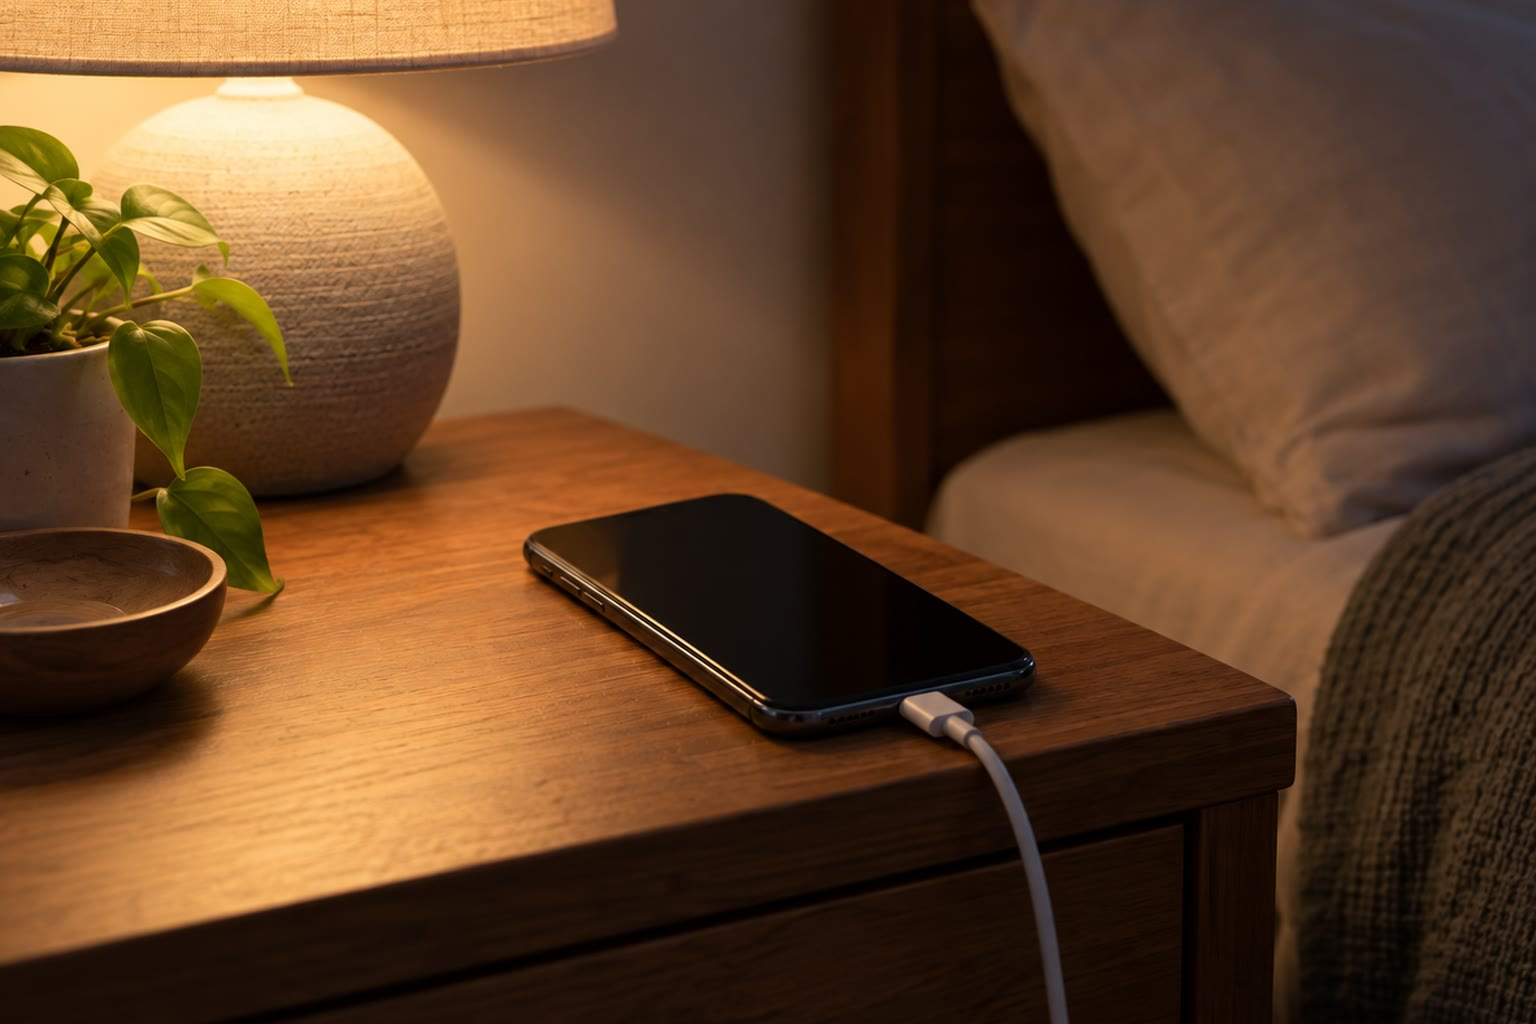
\includegraphics[width=0.45\linewidth]{images/book1/ai/g12-phone-charging.jpg}

{\small Mengisi daya ponsel: sebuah reaksi yang dipaksa berbalik arah
semalaman.}
\end{omfigure}

\section{Reaksi redoks yang dibelah dua}

Jika sebilah seng dicelupkan ke dalam larutan tembaga sulfat, seng
teroksidasi dan \omterm{def:g9:ions:ion}{ion-ion} tembaga tereduksi di permukaan bilah itu,
\ce{Zn + Cu^{2+} -> Zn^{2+} + Cu}: \omterm{def:g9:inside-the-atom:nucleus}{elektron-elektron} berpindah langsung
dari \omterm{def:g9:periodic-table-first-look:metal}{logam} ke \omterm{def:g9:ions:ion}{ion}, dan energinya hilang sebagai sedikit panas.
Pisahkanlah kedua bagian itu, lalu hubungkan dengan kawat: \omterm{def:g9:inside-the-atom:nucleus}{elektron} kini
harus berjalan melalui kawat, dan dapat menyalakan lampu di
perjalanannya.

\begin{definition}[Sel elektrokimia, setengah sel, jembatan garam]\label{def:g12:cells-and-electrolysis:cell}
Sebuah \emph{sel elektrokimia}\index{sel elektrokimia} menghasilkan
energi listrik dari \omterm{def:g11:redox:reaction}{reaksi redoks} yang \omterm{def:g11:redox:oxidation}{oksidasi} dan \omterm{def:g11:redox:oxidation}{reduksinya}
berlangsung di dua ruang yang terpisah. Setiap ruang, yaitu sebuah
elektrode \omterm{def:g9:periodic-table-first-look:metal}{logam} yang dicelupkan ke dalam larutan \omterm{def:g9:ions:ion}{ion-ionnya}, disebut
\emph{setengah sel}\index{setengah sel}. Sebuah
\emph{jembatan garam}\index{jembatan garam}, berupa tabung atau
secarik kertas yang dibasahi larutan \omterm{def:g9:ions:ion}{ion}, menghubungkan kedua larutan
dan menutup rangkaian sambil menjaga keduanya tetap terpisah.
\end{definition}

\begin{definition}[Anode, katode]\label{def:g12:cells-and-electrolysis:anode}
Elektrode tempat terjadinya \omterm{def:g11:redox:oxidation}{oksidasi} disebut \emph{anode}\index{anode};
elektrode tempat terjadinya \omterm{def:g11:redox:oxidation}{reduksi} disebut
\emph{katode}\index{katode}.
\end{definition}

\begin{omfigure}
\begin{tikzpicture}[font=\small, scale=1.25]
  \pic[transform shape] at (0,0) {beaker={0.7}{black!6}};
  \pic[transform shape] at (4,0) {beaker={0.7}{cyan!70!blue!35}};
  \pic[transform shape] (zn) at (-0.3,0.25) {electrode={black!30}};
  \pic[transform shape] (cu) at (4.3,0.25) {electrode={orange!70!brown}};
  \pic[transform shape] at (0.35,0.6) {saltbridge={3.3}};
  \pic[transform shape] (v) at (2,3.9) {meter={1.10 V}};
  \draw[black!70, thick] (zn-top) |- (1.0,3.4) -| (v-a);
  \draw[black!70, thick] (cu-top) |- (3.0,3.4) -| (v-b);
  \draw[->, omProp, very thick] (0.2,3.55) -- (1.0,3.55);
  \draw[->, omProp, very thick] (3.0,3.55) -- (3.8,3.55);
  \node[omProp, font=\footnotesize] at (0.6,3.75) {$e^-$};
  \node[omProp, font=\footnotesize] at (3.4,3.75) {$e^-$};
  \node[anchor=north, align=center] at (-0.2,-0.15) {anode ($-$): seng\\ \ce{Zn -> Zn^{2+} + 2e-}};
  \node[anchor=north, align=center] at (4.2,-0.15) {katode ($+$): tembaga\\ \ce{Cu^{2+} + 2e- -> Cu}};
  \node[font=\footnotesize, anchor=east, align=right] at (-0.95,0.7) {\ce{Zn^{2+}}\\ \ce{SO4^{2-}}};
  \node[font=\footnotesize, anchor=west, align=left] at (4.95,0.7) {\ce{Cu^{2+}}\\ \ce{SO4^{2-}}};
  \node[font=\footnotesize, align=center] at (2,2.45) {jembatan garam\\ (\ce{K+}, \ce{NO3-})};
\end{tikzpicture}

{\small Sel Daniell. \omterm{def:g9:inside-the-atom:nucleus}{Elektron} meninggalkan \omterm{def:g12:cells-and-electrolysis:anode}{anode} seng melalui kawat dan
memasuki \omterm{def:g12:cells-and-electrolysis:anode}{katode} tembaga; di dalam \omterm{def:g12:cells-and-electrolysis:cell}{jembatan garam}, \omterm{def:g9:ions:ion}{ion-ion} bergerak
untuk menjaga setiap larutan tetap netral.}
\end{omfigure}

\begin{proposition}[Ke mana elektron pergi]\label{prop:g12:cells-and-electrolysis:flow}
Dalam sel yang mengalirkan arus, \omterm{def:g9:inside-the-atom:nucleus}{elektron} meninggalkan sel melalui
\omterm{def:g12:cells-and-electrolysis:anode}{anode}, tempat \omterm{def:g9:inside-the-atom:nucleus}{elektron} dilepaskan oleh \omterm{def:g11:redox:oxidation}{oksidasi}, berjalan melalui
rangkaian luar, dan masuk melalui \omterm{def:g12:cells-and-electrolysis:anode}{katode}, tempat \omterm{def:g9:inside-the-atom:nucleus}{elektron} diterima oleh
\omterm{def:g11:redox:oxidation}{reduksi}. \omterm{def:g12:cells-and-electrolysis:anode}{Anode} adalah kutub negatif, \omterm{def:g12:cells-and-electrolysis:anode}{katode} kutub positif. Di dalam sel,
arus dibawa oleh \omterm{def:g9:ions:ion}{ion}: \omterm{def:g9:ions:ion}{kation} bergerak menuju \omterm{def:g12:cells-and-electrolysis:anode}{katode}, \omterm{def:g9:ions:ion}{anion} menuju
\omterm{def:g12:cells-and-electrolysis:anode}{anode}.
\end{proposition}

\begin{proof}
\omterm{def:g11:redox:oxidation}{Oksidasi} menghasilkan \omterm{def:g9:inside-the-atom:nucleus}{elektron} di \omterm{def:g12:cells-and-electrolysis:anode}{anode}; \omterm{def:g11:redox:oxidation}{reduksi} menghabiskannya di
\omterm{def:g12:cells-and-electrolysis:anode}{katode}; kawat adalah satu-satunya jalan di antara keduanya. Kalau tidak,
setiap larutan akan menjadi bermuatan, dan hal itu dicegah oleh \omterm{def:g9:ions:ion}{ion-ion}
\omterm{def:g12:cells-and-electrolysis:cell}{jembatan garam}.
\end{proof}

\begin{method}[Menguraikan sebuah sel]\label{met:g12:cells-and-electrolysis:describe}
\begin{enumerate}
  \item Tuliskan \omterm{def:g11:redox:reaction}{reaksi redoks} keseluruhan yang berlangsung spontan.
  \item Pecahlah reaksi itu menjadi dua \omterm{def:g11:redox:couple}{setengah reaksi}: \omterm{def:g11:redox:oxidation}{oksidasi}
        (\omterm{def:g12:cells-and-electrolysis:anode}{anode}) dan \omterm{def:g11:redox:oxidation}{reduksi} (\omterm{def:g12:cells-and-electrolysis:anode}{katode}).
  \item Tandai kutubnya: \omterm{def:g12:cells-and-electrolysis:anode}{anode} $-$, \omterm{def:g12:cells-and-electrolysis:anode}{katode} $+$; arah \omterm{def:g9:inside-the-atom:nucleus}{elektron} di dalam
        kawat (dari \omterm{def:g12:cells-and-electrolysis:anode}{anode} ke \omterm{def:g12:cells-and-electrolysis:anode}{katode}) dan arah arus (dari \omterm{def:g12:cells-and-electrolysis:anode}{katode} ke
        \omterm{def:g12:cells-and-electrolysis:anode}{anode}).
  \item Uraikan gerakan \omterm{def:g9:ions:ion}{ion-ion} di dalam \omterm{def:g12:cells-and-electrolysis:cell}{jembatan garam}.
\end{enumerate}
\end{method}


\begin{history}[Tumpukan Volta, 1800]
Pada tahun 1800 fisikawan Alessandro Volta menumpuk cakram-cakram dari
dua \omterm{def:g9:periodic-table-first-look:metal}{logam} yang berbeda, seng dan tembaga atau perak, yang dipisahkan
oleh potongan kain yang dibasahi air garam, dan memperoleh arus listrik
yang tetap: baterai pertama. Baterai itu memberi para fisikawan sumber
listrik kontinu yang pertama, dan para ahli kimia sebuah alat baru:
dalam beberapa tahun, \omterm{def:g12:cells-and-electrolysis:electrolysis}{elektrolisis} telah memisahkan natrium dan kalium
untuk pertama kalinya.
\end{history}

\begin{omfigure}
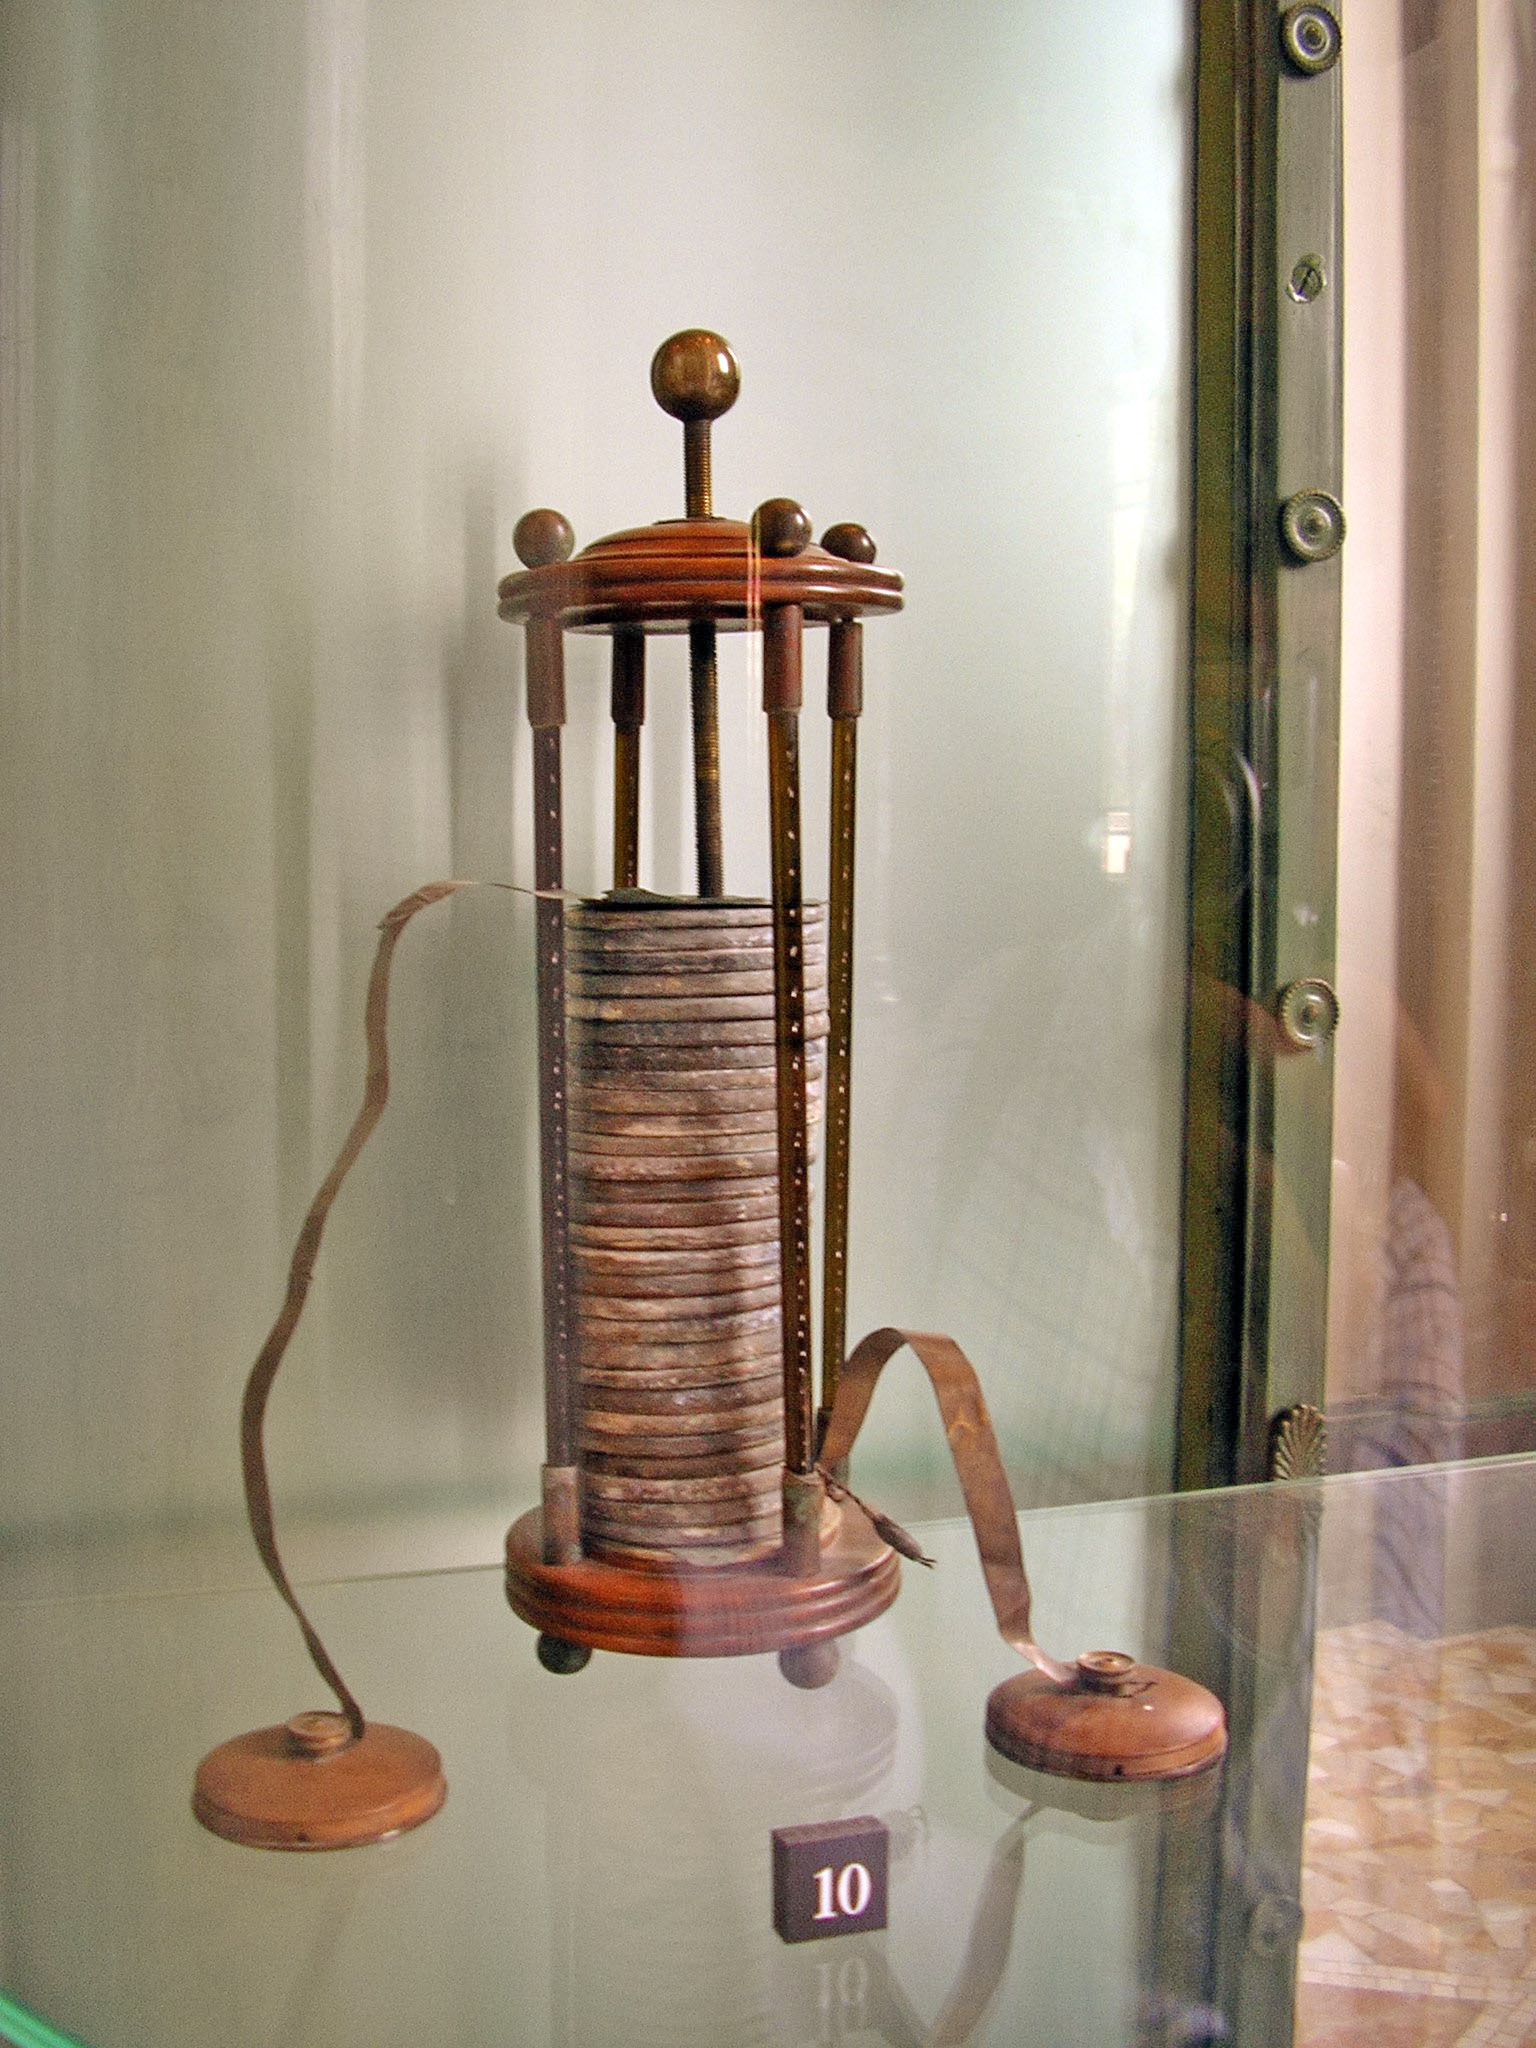
\includegraphics[width=0.24\linewidth]{images/book1/volta-pile.jpg}

{\small Tumpukan Volta di sebuah museum. Foto: GuidoB, CC\ BY-SA\ 3.0.}
\end{omfigure}

\section{Tegangan sel}

\begin{definition}[Tegangan sel]\label{def:g12:cells-and-electrolysis:emf}
Yang disebut \emph{tegangan sel}\index{tegangan sel} adalah tegangan
yang diukur di antara kutub-kutub sebuah sel yang tidak mengalirkan arus
(rangkaian terbuka), dengan voltmeter; nilainya positif jika kutub
positif voltmeter berada pada \omterm{def:g12:cells-and-electrolysis:anode}{katode}.
\end{definition}

\begin{example}[Sel Daniell]\label{ex:g12:cells-and-electrolysis:daniell}
% ledger: e0:Cu, e0:Zn, emf:Daniell
Dengan kedua larutan pada \qty{1}{mol/L}, sel Daniell memberikan
\qty{1.10}{V}. Cara meramalkan tegangan semacam itu dari tabel
potensial elektrode diperlihatkan dalam buku Tahun Pertama universitas.
\end{example}

\begin{remark}[Mengapa sel menjadi habis]\label{rem:g12:cells-and-electrolysis:runs-down}
Reaksi sel itu, \ce{Zn + Cu^{2+} -> Zn^{2+} + Cu}, memiliki tetapan $K$
yang sangat besar. Selama sel bekerja,
$Q = [\ce{Zn^{2+}}]/[\ce{Cu^{2+}}]$ bertambah, dan reaksinya terus
berlangsung selama $Q < K$. Jika sebuah \omterm{def:g7:chemical-reactions:reactant}{pereaksi} habis (seng, atau \omterm{def:g9:ions:ion}{ion}
tembaga), arusnya berhenti: sel itu ``habis''.
\end{remark}

\section{Muatan dan kapasitas}

\begin{definition}[Tetapan Faraday, kapasitas]\label{def:g12:cells-and-electrolysis:capacity}
Yang disebut \emph{tetapan Faraday}\index{tetapan Faraday} $F$ adalah
muatan listrik satu \omterm{def:g10:the-mole:amount}{mol} \omterm{def:g9:inside-the-atom:nucleus}{elektron}, $F = N_A e = \qty{96485}{C/mol}$.
Yang disebut \emph{kapasitas}\index{kapasitas} sebuah sel adalah muatan
listrik terbesar yang dapat dialirkannya, sering dinyatakan dalam
ampere-jam: $\qty{1}{A.h} = \qty{3600}{C}$.
\end{definition}

\begin{proposition}[Muatan dan jumlah elektron]\label{prop:g12:cells-and-electrolysis:charge}
% ledger: const:F, const:NA, const:e
Arus $I$ yang mengalir selama waktu $\Delta t$ membawa muatan
$Q = I\,\Delta t$, yaitu jumlah \omterm{def:g9:inside-the-atom:nucleus}{elektron}
\[
  n(e^-) = \frac{Q}{F} = \frac{I\,\Delta t}{F} .
\]
\end{proposition}

\begin{proof}
Setiap \omterm{def:g9:inside-the-atom:nucleus}{elektron} membawa muatan elementer $e$; $n$ \omterm{def:g10:the-mole:amount}{mol} \omterm{def:g9:inside-the-atom:nucleus}{elektron} membawa
$n N_A e = n F$.
\end{proof}

\begin{example}[Kapasitas sel Daniell]\label{ex:g12:cells-and-electrolysis:capacity}
% ledger: aw:Zn, const:F
Elektrode seng mengandung \qty{6.5}{g} seng yang dapat bereaksi, yaitu
$6.5/65.4 = \qty{0.099}{mol}$. Setiap \omterm{def:g7:atoms-and-molecules:atom}{atom} seng melepaskan dua
\omterm{def:g9:inside-the-atom:nucleus}{elektron}: $n(e^-) = \qty{0.199}{mol}$, jadi
$Q = 0.199 \times 96485 = \qty{1.9e4}{C}$, sekitar
$\qty{1.9e4}{}/3600 = \qty{5.3}{A.h}$, jika \omterm{def:g9:ions:ion}{ion-ion} tembaga tidak habis
lebih dahulu.
\end{example}

\section{Elektrolisis}

\begin{definition}[Elektrolisis, akumulator]\label{def:g12:cells-and-electrolysis:electrolysis}
Yang disebut \emph{elektrolisis}\index{elektrolisis} adalah \omterm{def:g11:redox:reaction}{reaksi
redoks} yang dipaksa oleh sebuah generator listrik, ke arah yang
berlawanan dengan arah yang akan diambilnya dengan sendirinya. Yang
disebut \emph{akumulator}\index{akumulator} adalah sel yang dapat diisi
ulang: selama pengisian, generator memaksa reaksinya berbalik arah,
sebagai sebuah elektrolisis.
\end{definition}

\begin{inthelab}[Elektrolisis air]
Dua elektrode dicelupkan ke dalam air yang dibuat dapat menghantarkan
listrik dengan sedikit natrium sulfat, masing-masing di bawah sebuah
tabung reaksi terbalik yang penuh berisi larutan itu. Dengan generator
beberapa volt, gelembung-gelembung naik dari kedua elektrode: di \omterm{def:g12:cells-and-electrolysis:anode}{katode}
(yang terhubung ke kutub $-$) gas hidrogen, di \omterm{def:g12:cells-and-electrolysis:anode}{anode} gas oksigen, dengan
gas yang pertama dua kali lebih banyak daripada yang kedua. Bilah kayu
yang menyala menimbulkan letupan dalam gas pertama; bilah kayu berbara
menyala kembali dalam gas kedua.
\end{inthelab}

\begin{omfigure}
\begin{tikzpicture}[font=\small, scale=1.2]
  % a trough of water, two inverted tubes standing in it
  \fill[omWater] (-1.4,0) rectangle (1.4,1.1);
  \foreach \x/\g in {-0.6/1.2, 0.6/0.6} {
    \fill[omWater] (\x-0.18,0.3) rectangle (\x+0.18,2.9);
    \fill[white] (\x-0.18,{2.9-\g}) rectangle (\x+0.18,2.9);
    \fill[white] (\x,2.9) circle (0.18);
    \draw[om glass] (\x-0.18,0.3) -- (\x-0.18,2.9) arc[start angle=180, end angle=0, radius=0.18] -- (\x+0.18,0.3);
  }
  \draw[om glass] (-1.5,1.25) -- (-1.4,1.15) -- (-1.4,0) -- (1.4,0) -- (1.4,1.15) -- (1.5,1.25);
  \fill[black!55] (-0.65,0) rectangle (-0.55,0.6);
  \fill[black!55] (0.55,0) rectangle (0.65,0.6);
  \node[draw, fill=white, minimum width=1.6cm, minimum height=0.45cm, font=\footnotesize] (g) at (0,-0.75) {generator};
  \draw[black!70, thick] (-0.6,0) -- (-0.6,0 |- g.north);
  \draw[black!70, thick] (0.6,0) -- (0.6,0 |- g.north);
  \node[font=\footnotesize] at (-0.78,-0.3) {$-$};
  \node[font=\footnotesize] at (0.78,-0.3) {$+$};
  \node[anchor=east, align=right] at (-0.95,2.5) {gas hidrogen\\ (katode)};
  \node[anchor=west, align=left] at (0.95,2.5) {gas oksigen\\ (anode)};
\end{tikzpicture}

{\small \omterm{def:g12:cells-and-electrolysis:electrolysis}{Elektrolisis} air: gas hidrogen yang terkumpul di atas elektrode
dua kali lebih banyak daripada gas oksigen.}
\end{omfigure}


\begin{example}[Air yang dipecah]\label{ex:g12:cells-and-electrolysis:water}
Di \omterm{def:g12:cells-and-electrolysis:anode}{katode}: \ce{2H2O + 2e- -> H2 + 2OH-}; di \omterm{def:g12:cells-and-electrolysis:anode}{anode}:
\ce{6H2O -> O2 + 4H3O+ + 4e-}. Untuk empat \omterm{def:g9:inside-the-atom:nucleus}{elektron}, terbentuk dua
\omterm{def:g7:atoms-and-molecules:molecule}{molekul} hidrogen dan satu \omterm{def:g7:atoms-and-molecules:molecule}{molekul} oksigen, sementara \omterm{def:g9:ions:ion}{ion} \ce{H3O+} dan
\ce{OH-} yang terbentuk di kedua elektrode bergabung kembali menjadi
air: secara keseluruhan \ce{2H2O -> 2H2 + O2}, kebalikan dari
\omterm{def:g4:what-a-fire-needs:burning}{pembakaran} hidrogen, yang memerlukan energi agar dapat terjadi.
\end{example}

\begin{method}[Massa yang diendapkan elektrolisis]\label{met:g12:cells-and-electrolysis:mass}
\begin{enumerate}
  \item Tuliskan \omterm{def:g11:redox:couple}{setengah reaksi} di elektrode tempat \omterm{def:g9:periodic-table-first-look:metal}{logam} terbentuk,
        misalnya \ce{Cu^{2+} + 2e- -> Cu}.
  \item Hitung muatan $Q = I \Delta t$ dan $n(e^-) = Q/F$.
  \item Bagilah dengan jumlah \omterm{def:g9:inside-the-atom:nucleus}{elektron} per \omterm{def:g7:atoms-and-molecules:atom}{atom}: $n(\ce{Cu}) =
        n(e^-)/2$; lalu $m = n \times M$.
\end{enumerate}
\end{method}


\begin{example}[Pemurnian tembaga]\label{ex:g12:cells-and-electrolysis:refining}
% ledger: aw:Cu, const:F
Tembaga tak murni dari tanur peleburan dijadikan \omterm{def:g12:cells-and-electrolysis:anode}{anode} sebuah sel
\omterm{def:g12:cells-and-electrolysis:electrolysis}{elektrolisis} dalam larutan tembaga sulfat, dan selembar tipis tembaga
murni dijadikan \omterm{def:g12:cells-and-electrolysis:anode}{katodenya}. Di \omterm{def:g12:cells-and-electrolysis:anode}{anode}, tembaga \omterm{def:g2:mixing-and-dissolving:dissolve}{larut},
\ce{Cu -> Cu^{2+} + 2e-}; di \omterm{def:g12:cells-and-electrolysis:anode}{katode}, tembaga murni diendapkan,
\ce{Cu^{2+} + 2e- -> Cu}; pengotornya jatuh ke dasar atau tetap dalam
larutan. Arus \qty{100}{A} selama \qty{24}{h} membawa
$Q = 100 \times 86400 = \qty{8.64e6}{C}$, yaitu
$n(e^-) = \qty{89.5}{mol}$, yang mengendapkan
$89.5/2 = \qty{44.8}{mol}$ tembaga: \qty{2.84}{kg}.
\end{example}

\begin{omfigure}
\begin{tikzpicture}[font=\small, scale=1.25]
  \pic[transform shape] at (0,0) {beaker={0.75}{cyan!70!blue!35}};
  \pic[transform shape] (an) at (-0.4,0.2) {electrode={orange!40!brown!80!black}};
  \pic[transform shape] (ca) at (0.4,0.2) {electrode={orange!80!brown}};
  \foreach \p in {(-0.6,0.08),(-0.5,0.12),(-0.3,0.07),(-0.2,0.1)} \fill[black!55] \p circle (0.03);
  \node[draw, fill=white, font=\footnotesize, minimum width=1.6cm] (g) at (0,3.4) {generator};
  \draw[black!70, thick] (an-top) -- (an-top |- g.south);
  \draw[black!70, thick] (ca-top) -- (ca-top |- g.south);
  \node[font=\footnotesize] at (-0.58,2.95) {$+$};
  \node[font=\footnotesize] at (0.58,2.95) {$-$};
  \draw[omProp, thick, <-] (-0.55,1.2) -- (-1.6,1.6) node[left, align=right, text=black] {anode tembaga\\ tak murni: larut};
  \draw[omProp, thick, <-] (0.55,1.2) -- (1.6,1.6) node[right, align=left, text=black] {katode tembaga\\ murni: bertambah};
  \draw[omProp, thick, <-] (-0.35,0.1) -- (-1.6,0.3) node[left, text=black] {pengotor};
\end{tikzpicture}

{\small Pemurnian tembaga dengan \omterm{def:g12:cells-and-electrolysis:electrolysis}{elektrolisis}: tembaga berpindah dari
\omterm{def:g12:cells-and-electrolysis:anode}{anode} yang tak murni ke \omterm{def:g12:cells-and-electrolysis:anode}{katode} yang murni melalui larutan.}
\end{omfigure}

\section{Baterai, akumulator, dan sel bahan bakar}

Setiap baterai adalah sel, setiap baterai isi ulang adalah \omterm{def:g12:cells-and-electrolysis:electrolysis}{akumulator}.
Aki timbal--asam pada mobil bekerja dengan timbal, timbal oksida, dan
asam sulfat; \omterm{def:g12:cells-and-electrolysis:electrolysis}{akumulator} litium-ion pada ponsel memindahkan \omterm{def:g9:ions:ion}{ion-ion}
litium di antara dua elektrode, yang satu dari grafit dan yang lain dari
oksida \omterm{def:g9:periodic-table-first-look:metal}{logam}, melalui elektrolit cair atau polimer, sementara
\omterm{def:g9:inside-the-atom:nucleus}{elektron-elektronnya} berputar melalui rangkaian luar. Sel \omterm{def:g4:what-a-fire-needs:fuel}{bahan bakar}
adalah sel yang \omterm{def:g7:chemical-reactions:reactant}{pereaksinya} dimasukkan terus-menerus: sel \omterm{def:g4:what-a-fire-needs:fuel}{bahan bakar}
hidrogen menjalankan reaksi \ce{2H2 + O2 -> 2H2O}, kebalikan dari
\omterm{def:g12:cells-and-electrolysis:electrolysis}{elektrolisis} air, dan menghasilkan listrik dan air. Gas hidrogen yang
dibuat dengan \omterm{def:g12:cells-and-electrolysis:electrolysis}{elektrolisis} memakai listrik dari angin atau matahari,
lalu dipakai dalam sel \omterm{def:g4:what-a-fire-needs:fuel}{bahan bakar}, adalah salah satu cara menyimpan
listrik itu.

\begin{omfigure}
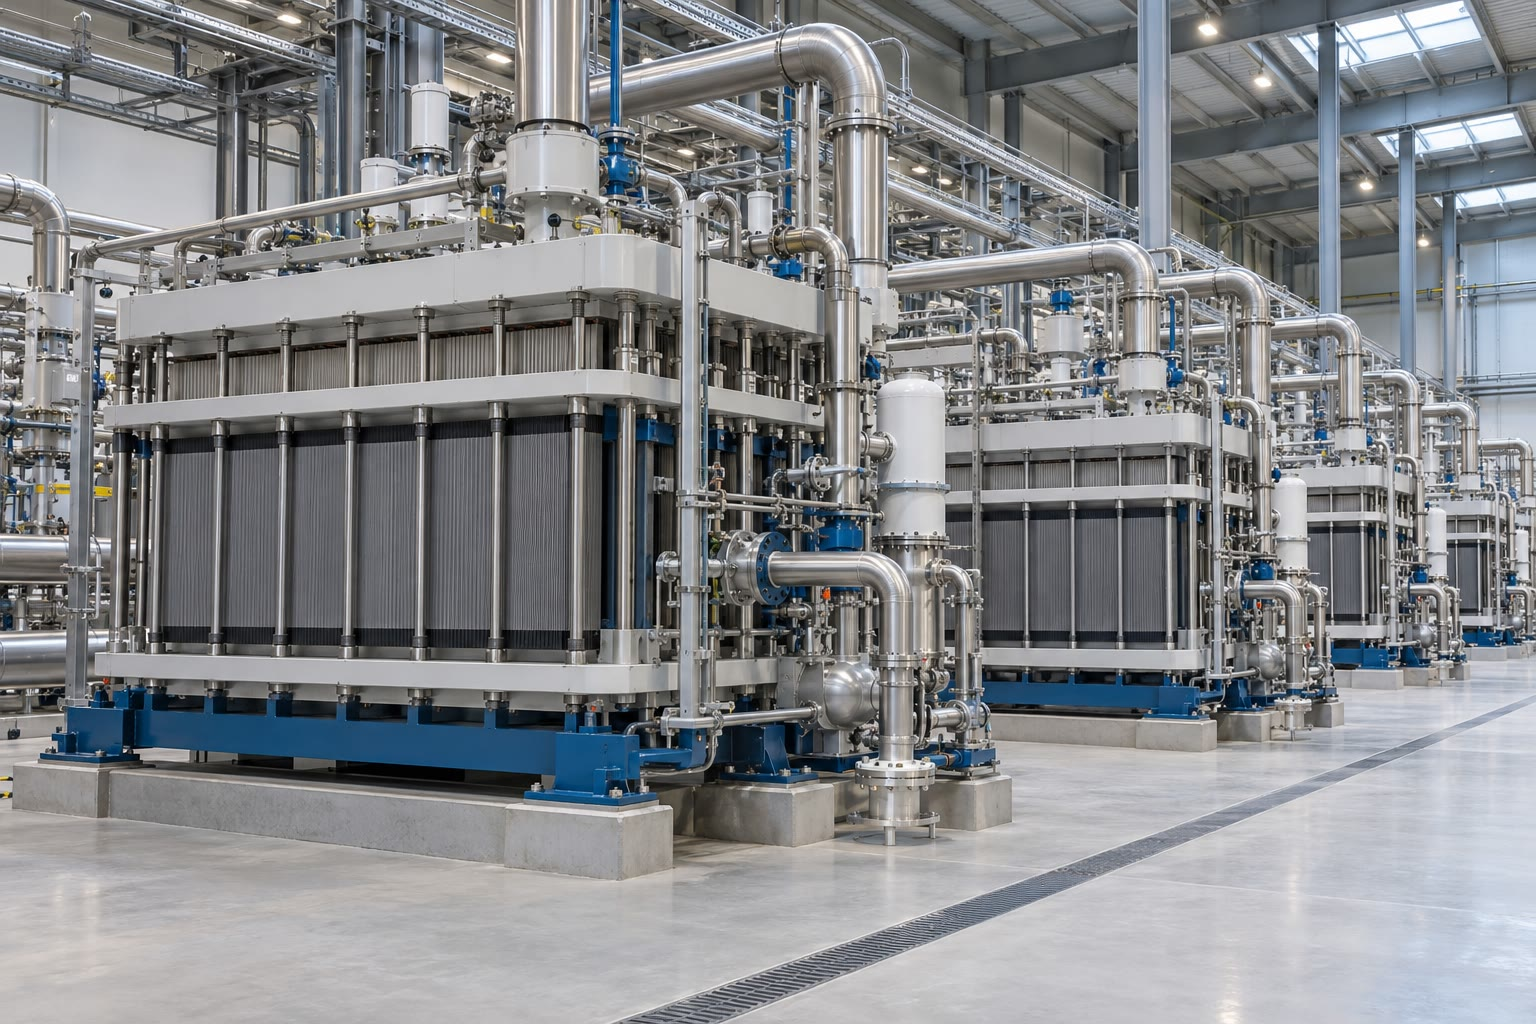
\includegraphics[width=0.48\linewidth]{images/book1/ai/g12-electrolyser-hall.jpg}

{\small Aula elektroliser: air dipecah menjadi gas hidrogen dan gas
oksigen.}
\end{omfigure}

\section{Latihan}

\begin{exercise}[$\star$]\label{exo:g12:cells-and-electrolysis:1}
Pada sel Daniell, elektrode mana yang menjadi \omterm{def:g12:cells-and-electrolysis:anode}{anode}? \omterm{def:g12:cells-and-electrolysis:anode}{Katode}? Tuliskan
\omterm{def:g11:redox:couple}{setengah reaksi} pada masing-masing elektrode.
\end{exercise}

\begin{exercise}[$\star$]\label{exo:g12:cells-and-electrolysis:2}
Arus \qty{0.20}{A} mengalir selama \qty{30}{min}. Hitung muatan yang
dibawa dan jumlah \omterm{def:g9:inside-the-atom:nucleus}{elektronnya}.
\end{exercise}

\begin{exercise}[$\star$]\label{exo:g12:cells-and-electrolysis:3}
Apa peran \omterm{def:g12:cells-and-electrolysis:cell}{jembatan garam}? Apa yang terjadi jika jembatan itu dilepas?
\end{exercise}

\begin{exercise}[$\star$]\label{exo:g12:cells-and-electrolysis:4}
Ubahlah \omterm{def:g12:cells-and-electrolysis:capacity}{kapasitas} \qty{2.5}{A.h} menjadi coulomb.
\end{exercise}

\begin{exercise}[$\star$]\label{exo:g12:cells-and-electrolysis:5}
Dalam \omterm{def:g12:cells-and-electrolysis:electrolysis}{elektrolisis}, apakah reaksinya spontan? Apa yang memasok
energinya?
\end{exercise}

\begin{exercise}[$\star\star$]\label{exo:g12:cells-and-electrolysis:6}
Sebuah sel dibuat dari elektrode perak dalam perak nitrat dan elektrode
tembaga dalam tembaga sulfat. Voltmeter menunjukkan bahwa \omterm{def:g9:inside-the-atom:nucleus}{elektron}
meninggalkan sel melalui tembaga. Tuliskan \omterm{def:g11:redox:couple}{setengah reaksinya},
sebutkan \omterm{def:g12:cells-and-electrolysis:anode}{anode} dan \omterm{def:g12:cells-and-electrolysis:anode}{katodenya}, dan berikan reaksi keseluruhannya.
\end{exercise}

\begin{exercise}[$\star\star$]\label{exo:g12:cells-and-electrolysis:7}
Sebuah baterai jam tangan mengalirkan \qty{10}{\micro A} terus-menerus
selama tiga tahun. Berapa \omterm{def:g12:cells-and-electrolysis:capacity}{kapasitasnya} dalam \si{mA.h}?
\end{exercise}

\begin{exercise}[$\star\star$]\label{exo:g12:cells-and-electrolysis:8}
Sebuah sendok dilapisi perak dengan arus \qty{0.50}{A} selama
\qty{40}{min}, \ce{Ag+ + e- -> Ag}. Berapa massa perak yang diendapkan?
\end{exercise}

\begin{exercise}[$\star\star$]\label{exo:g12:cells-and-electrolysis:9}
Pada gambar sel Daniell, tentukan arah arus di dalam kawat, dan arah
gerak \omterm{def:g9:ions:ion}{ion-ion} \ce{K+} dan \ce{NO3-} di dalam \omterm{def:g12:cells-and-electrolysis:cell}{jembatan garam}.
\end{exercise}

\begin{exercise}[$\star\star$]\label{exo:g12:cells-and-electrolysis:10}
Bandingkan sel dan \omterm{def:g12:cells-and-electrolysis:electrolysis}{elektrolisis}: tanda \omterm{def:g12:cells-and-electrolysis:anode}{anode}, arah reaksi, dan
perubahan bentuk energinya.
\end{exercise}

\begin{exercise}[$\star\star$]\label{exo:g12:cells-and-electrolysis:11}
Dalam \omterm{def:g12:cells-and-electrolysis:electrolysis}{elektrolisis} air, \qty{24}{mL} gas hidrogen terkumpul. Berapa
volume gas oksigen yang terkumpul pada waktu yang sama? Mengapa?
\end{exercise}

\begin{exercise}[$\star\star\star$]\label{exo:g12:cells-and-electrolysis:12}
Sebuah sel Daniell mengandung \qty{5.0}{g} seng dan \qty{100}{mL}
tembaga sulfat \qty{0.50}{mol/L}. \omterm{def:g7:chemical-reactions:reactant}{Pereaksi} mana yang habis lebih
dahulu? Berapa \omterm{def:g12:cells-and-electrolysis:capacity}{kapasitas} sel itu? Berapa lama sel itu dapat mengalirkan
\qty{50}{mA}?
\end{exercise}

\begin{exercise}[$\star\star\star$]\label{exo:g12:cells-and-electrolysis:13}
Sebuah baterai \qty{1.5}{V} mengalirkan \qty{2.0}{A.h}. Hitung energi
yang disimpannya ($E = Q U$), dalam joule dan dalam watt-jam.
\end{exercise}

\begin{exercise}[$\star\star\star$]\label{exo:g12:cells-and-electrolysis:14}
Air dielektrolisis dengan \qty{2.0}{A} selama \qty{1.0}{h}. Hitung
jumlah, lalu volume pada \qty{20}{\celsius} ($V_m = \qty{24.1}{L/mol}$),
gas hidrogen dan gas oksigen yang dihasilkan.
\end{exercise}

\begin{exercise}[$\star\star\star$]\label{exo:g12:cells-and-electrolysis:15}
Pada pemurnian tembaga, \omterm{def:g12:cells-and-electrolysis:anode}{anode} kehilangan \qty{3.00}{kg} bahan sementara
\omterm{def:g12:cells-and-electrolysis:anode}{katode} bertambah \qty{2.84}{kg} tembaga. Berapa persentase tembaga
dalam \omterm{def:g12:cells-and-electrolysis:anode}{anode} yang tak murni itu, dengan menganggap bahwa hanya tembaga
yang teroksidasi di \omterm{def:g12:cells-and-electrolysis:anode}{anode} dan pengotornya hanya berjatuhan?
\end{exercise}

\section{Soal: Baterai Ponsel}

\begin{problem}[{Soal akhir pekan --- berapa massa litium yang bolak-balik
di antara elektrode-elektrode baterai ponsel \qty{4000}{mA.h}?}]
\label{pb:g12:cells-and-electrolysis:1}
% ledger: const:F, const:NA, aw:Li, dch:CH4, aw:C, aw:H
Sebuah baterai ponsel berlabel ``\qty{3.7}{V}, \qty{4000}{mA.h}''.
Dalam gambaran yang disederhanakan, selama pengosongan setiap \omterm{def:g7:atoms-and-molecules:atom}{atom}
litium yang tersimpan dalam elektrode grafit melepaskan satu \omterm{def:g9:inside-the-atom:nucleus}{elektron}
dan keluar sebagai \omterm{def:g9:ions:ion}{ion} litium, \ce{Li -> Li+ + e-}; \omterm{def:g9:ions:ion}{ion} itu menyeberangi
elektrolit dan diterima oleh elektrode oksida \omterm{def:g9:periodic-table-first-look:metal}{logam}, yang pada saat yang
sama menerima sebuah \omterm{def:g9:inside-the-atom:nucleus}{elektron}.

\medskip
\noindent\textbf{Bagian I --- Selnya.}
\begin{enumerate}
  \item Selama pengosongan, apakah elektrode grafit merupakan \omterm{def:g12:cells-and-electrolysis:anode}{anode} atau
        \omterm{def:g12:cells-and-electrolysis:anode}{katode}? Mengapa?
  \item Kutub mana yang negatif?
  \item Ke arah mana \omterm{def:g9:inside-the-atom:nucleus}{elektron} berjalan melalui ponsel? Dan \omterm{def:g9:ions:ion}{ion-ion}
        litium di dalam baterai?
  \item Mengapa sel ini merupakan \omterm{def:g12:cells-and-electrolysis:electrolysis}{akumulator}?
\end{enumerate}

\medskip
\noindent\textbf{Bagian II --- Muatannya.}
\begin{enumerate}[resume]
  \item Ubahlah \qty{4000}{mA.h} menjadi ampere-jam, lalu menjadi
        coulomb.
  \item Hitung jumlah \omterm{def:g9:inside-the-atom:nucleus}{elektron} yang diwakili muatan ini.
  \item Berapa banyak \omterm{def:g9:inside-the-atom:nucleus}{elektron} itu?
  \item Ponsel itu rata-rata menarik arus \qty{0.25}{A}. Berapa lama
        baterai yang penuh dapat bertahan?
  \item Layarnya menunjukkan 20 \%. Berapa muatan, dalam coulomb, yang
        tersisa?
\end{enumerate}

\medskip
\noindent\textbf{Bagian III --- Energinya.}
\begin{enumerate}[resume]
  \item Hitung energi yang tersimpan, $E = Q U$, dalam joule.
  \item Ubahlah menjadi watt-jam.
  \item Bandingkan dengan energi yang dilepaskan oleh \omterm{def:g4:what-a-fire-needs:burning}{pembakaran}
        \qty{1}{g} metana (\qty{55.7}{kJ}).
  \item Berapa kali pengisian penuh yang diberikan \qty{1}{kW.h}
        listrik, jika tidak ada energi yang hilang?
\end{enumerate}

\medskip
\noindent\textbf{Bagian IV --- Pengisian ulang.}
\begin{enumerate}[resume]
  \item Selama pengisian, reaksi apa yang terjadi di elektrode grafit?
        Apakah reaksi itu \omterm{def:g11:redox:oxidation}{oksidasi} atau \omterm{def:g11:redox:oxidation}{reduksi}?
  \item Mengapa pengisian ulang merupakan \omterm{def:g12:cells-and-electrolysis:electrolysis}{elektrolisis}?
  \item Pengisi dayanya mengalirkan \qty{2.0}{A}. Paling cepat berapa
        lama pengisian ulang penuh berlangsung?
  \item Berapa jumlah \omterm{def:g9:ions:ion}{ion} litium yang menyeberangi elektrolit selama
        satu pengisian penuh?
  \item Hitung massanya.
  \item Nyatakan jawaban akhirnya: berapa massa litium yang bolak-balik
        di antara elektrode-elektrode dalam satu pengisian penuh?
\end{enumerate}
\end{problem}
